%================================================================
\section{Introduction}
%================================================================
In this course, we will conduct a propulsion design analysis by considering three different propulsion systems, namely (i) a propeller-driven internal combustion engine, (ii) a turbojet engine, and (iii) a single-stage liquid rocket engine. Performance, efficiency, and other characteristics (emissions, fuel-utilization, and noise, etc) will be investigated in the specific context of a small four-seat private aircraft (similar to the Cirrus SR-22). The aircraft is illustrated in \cref{FIG_CIRRUS} and aircraft specifications are summarized in \cref{TAB_CIRRUS_SPECS}. The primary focus of this course is on the engine design analysis of gas turbines with specific consideration of  turbojet and turbofan engines. 

%================================================================
\begin{figure}[!tbh!]
  \begin{floatrow}
    \ffigbox{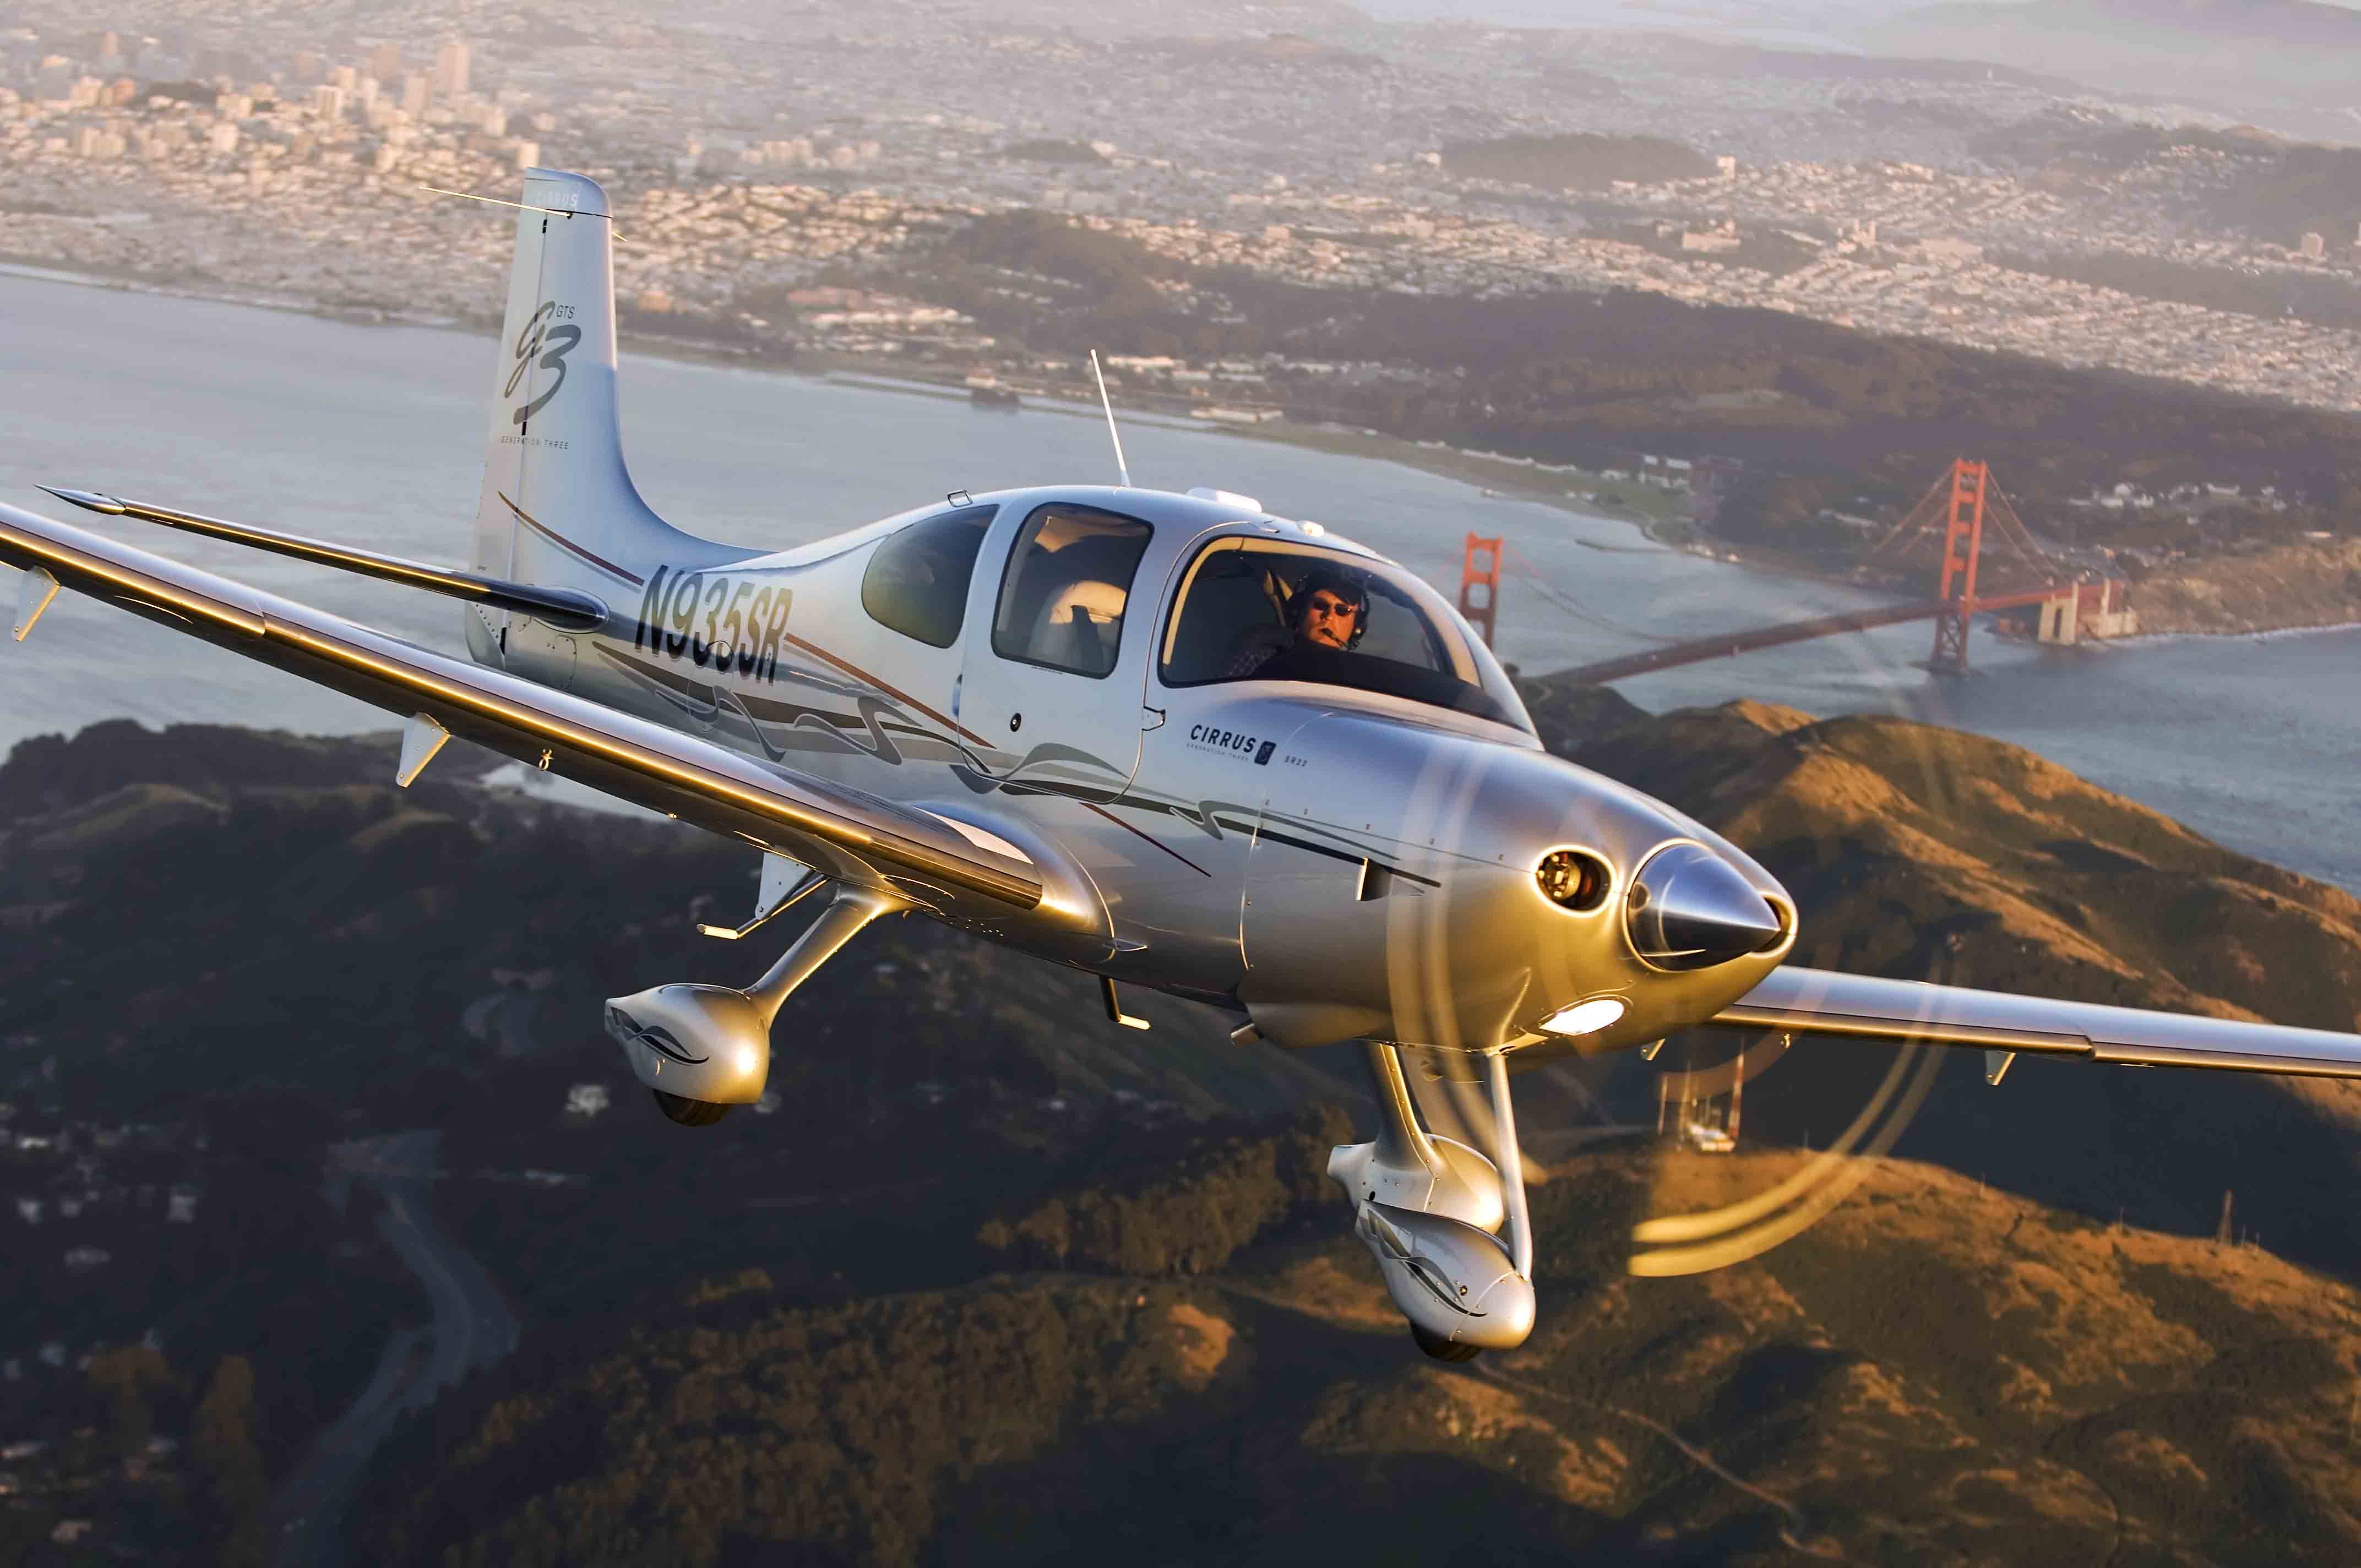
\includegraphics[width=0.56\textwidth]{cirrusSR22_photo1}}{\caption{\label{FIG_CIRRUS}Cirrus SR22.}}
    \capbtabbox{
      \begin{tabular}{|lc|}
        \hline
        \multicolumn{2}{|c|}{Performance}\\\hline\hline
        Climb Rate & 6.45 m/s\\
        Max. operating altitude & 5,334 m\\
        Max. cruise speed & 340 km/h\\\hline\hline
        \multicolumn{2}{|c|}{Weight Certification}\\\hline\hline
        Max. takeoff mass & 1542 kg\\
        Empty mass     & 1021 kg\\
        Maximum load       & 521 kg\\
        Full fuel payload         & 307 kg\\\hline\hline
        \multicolumn{2}{|c|}{Wings}\\\hline\hline
        Wing span     & 11.67 m\\
        Wing area & 13.5 m$^2$\\\hline
      \end{tabular}
    }{\caption{\label{TAB_CIRRUS_SPECS}Specifications of Cirrus SR22.}}
  \end{floatrow}
\end{figure}
%================================================================

The following specific engine design concepts are of interest for aircraft engines:
\begin{itemize}
\item {Scenario 1: Internal combustion engine}
  \begin{itemize}[noitemsep,topsep=0pt]
    \item Propeller-driven IC-engine;
    \item Single six-cylinder four-stroke engine;
    \item Example: Cessna 350 Corvalis (\cref{FIG_EXAMPLE_CESSNA}); engine:  Teledyne Continental IO-550-N.
  \end{itemize}
\item {Scenario 2: Gas-turbine engine}
  \begin{itemize}[noitemsep,topsep=0pt]
    \item Turbo-fan engine;
    \item Two-stage compressor/turbine;
    \item Example: Honda HA-420 HondaJet (\cref{FIG_EXAMPLE_HONDA}); engine: GE Honda HF120.
  \end{itemize}
\item {Scenario 3: Rocket-propelled engine}
  \begin{itemize}[noitemsep,topsep=0pt]
    \item Single-stage rocket booster;
    \item Fuels: solid, liquid, hybrid fuels;
    \item Example: Messerschmitt Me 163 (\cref{FIG_EXAMPLE_ME163}); engine: HWK 109Ð509.
  \end{itemize}
\end{itemize}

%==============================================================================
\begin{figure}[!tbh!]
  \begin{center}
  \begin{subfigmatrix}{1}
   \subfigure[\label{FIG_EXAMPLE_CESSNA}Cessna 350 Corvalis.]{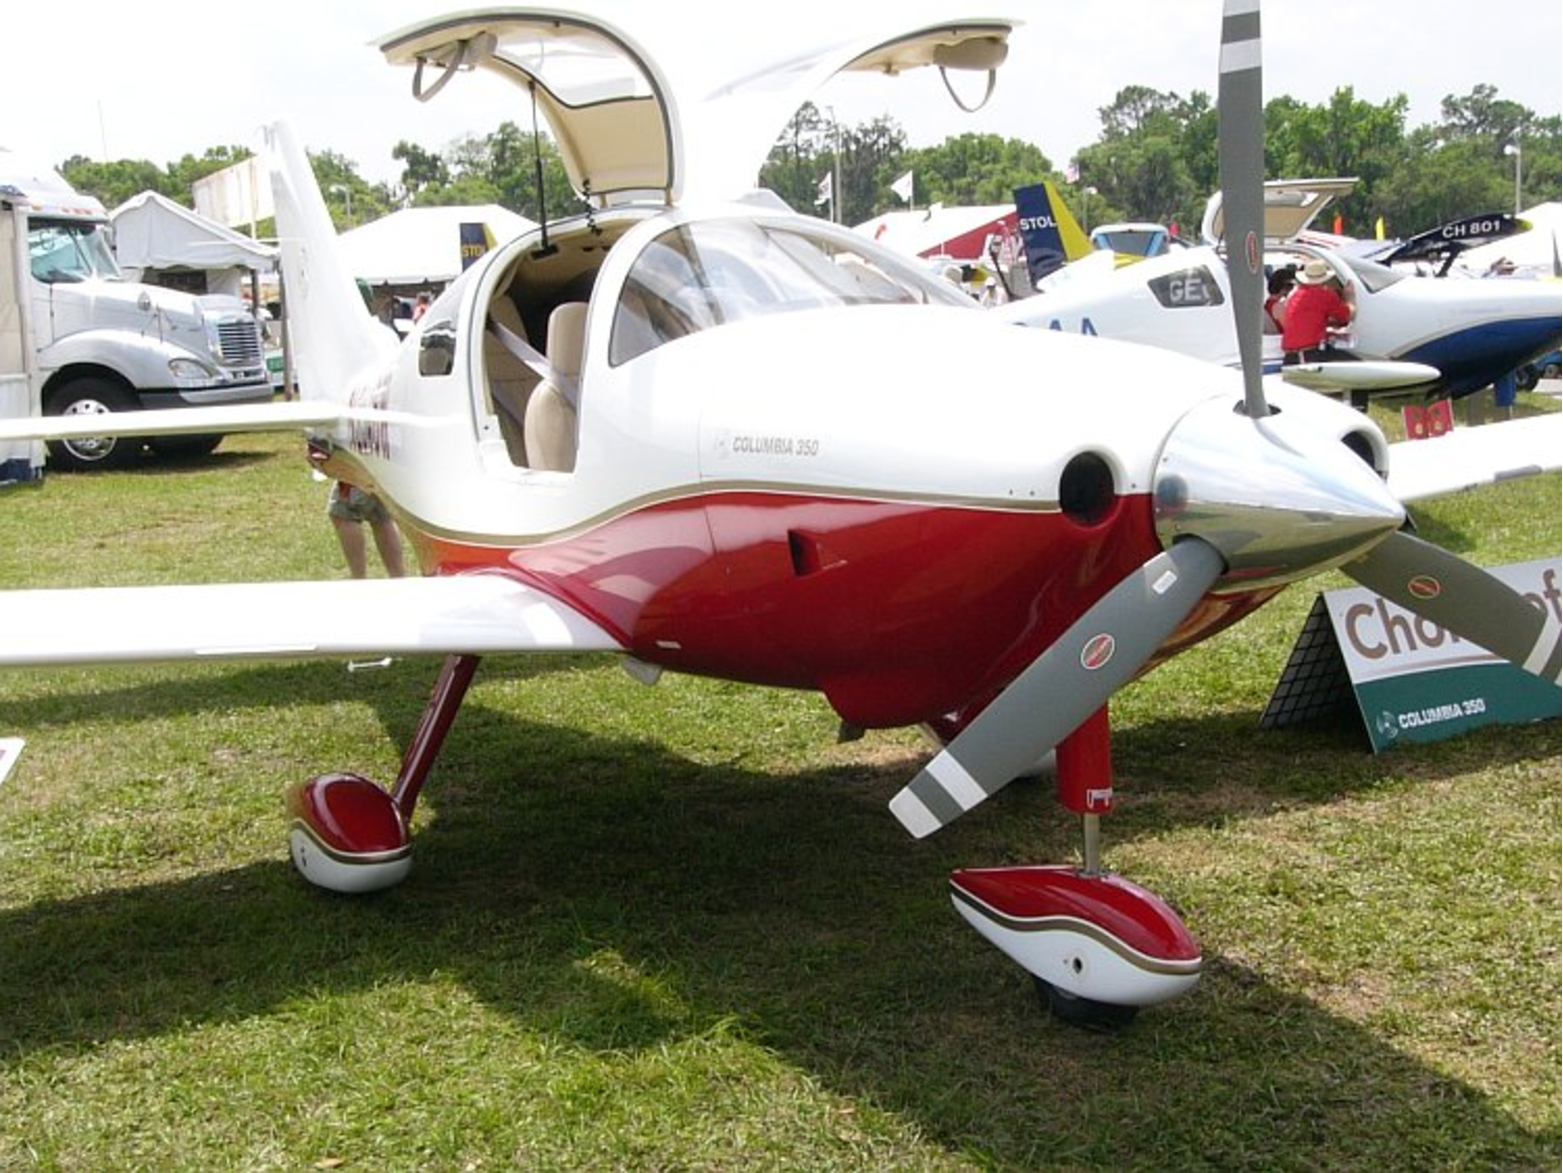
\includegraphics[width = 0.45\textwidth,clip=]{cessna}}
   \subfigure[\label{FIG_EXAMPLE_HONDA}Honda HA-420 HondaJet.]{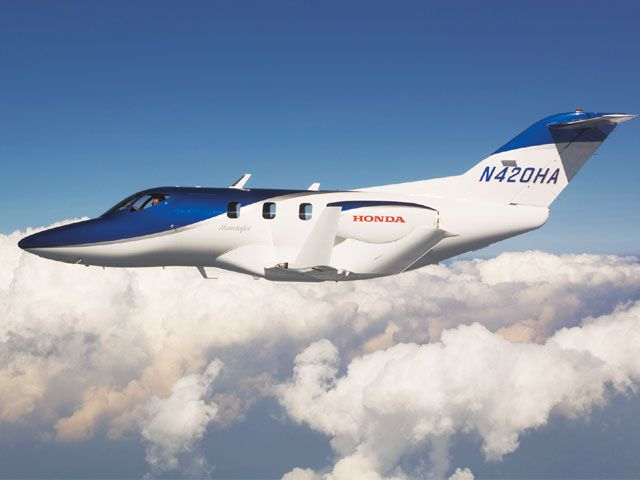
\includegraphics[width = 0.45\textwidth,clip=]{HondaJet_Side}}
   \subfigure[\label{FIG_EXAMPLE_ME163}Messerschmitt ME-163 Komet.]{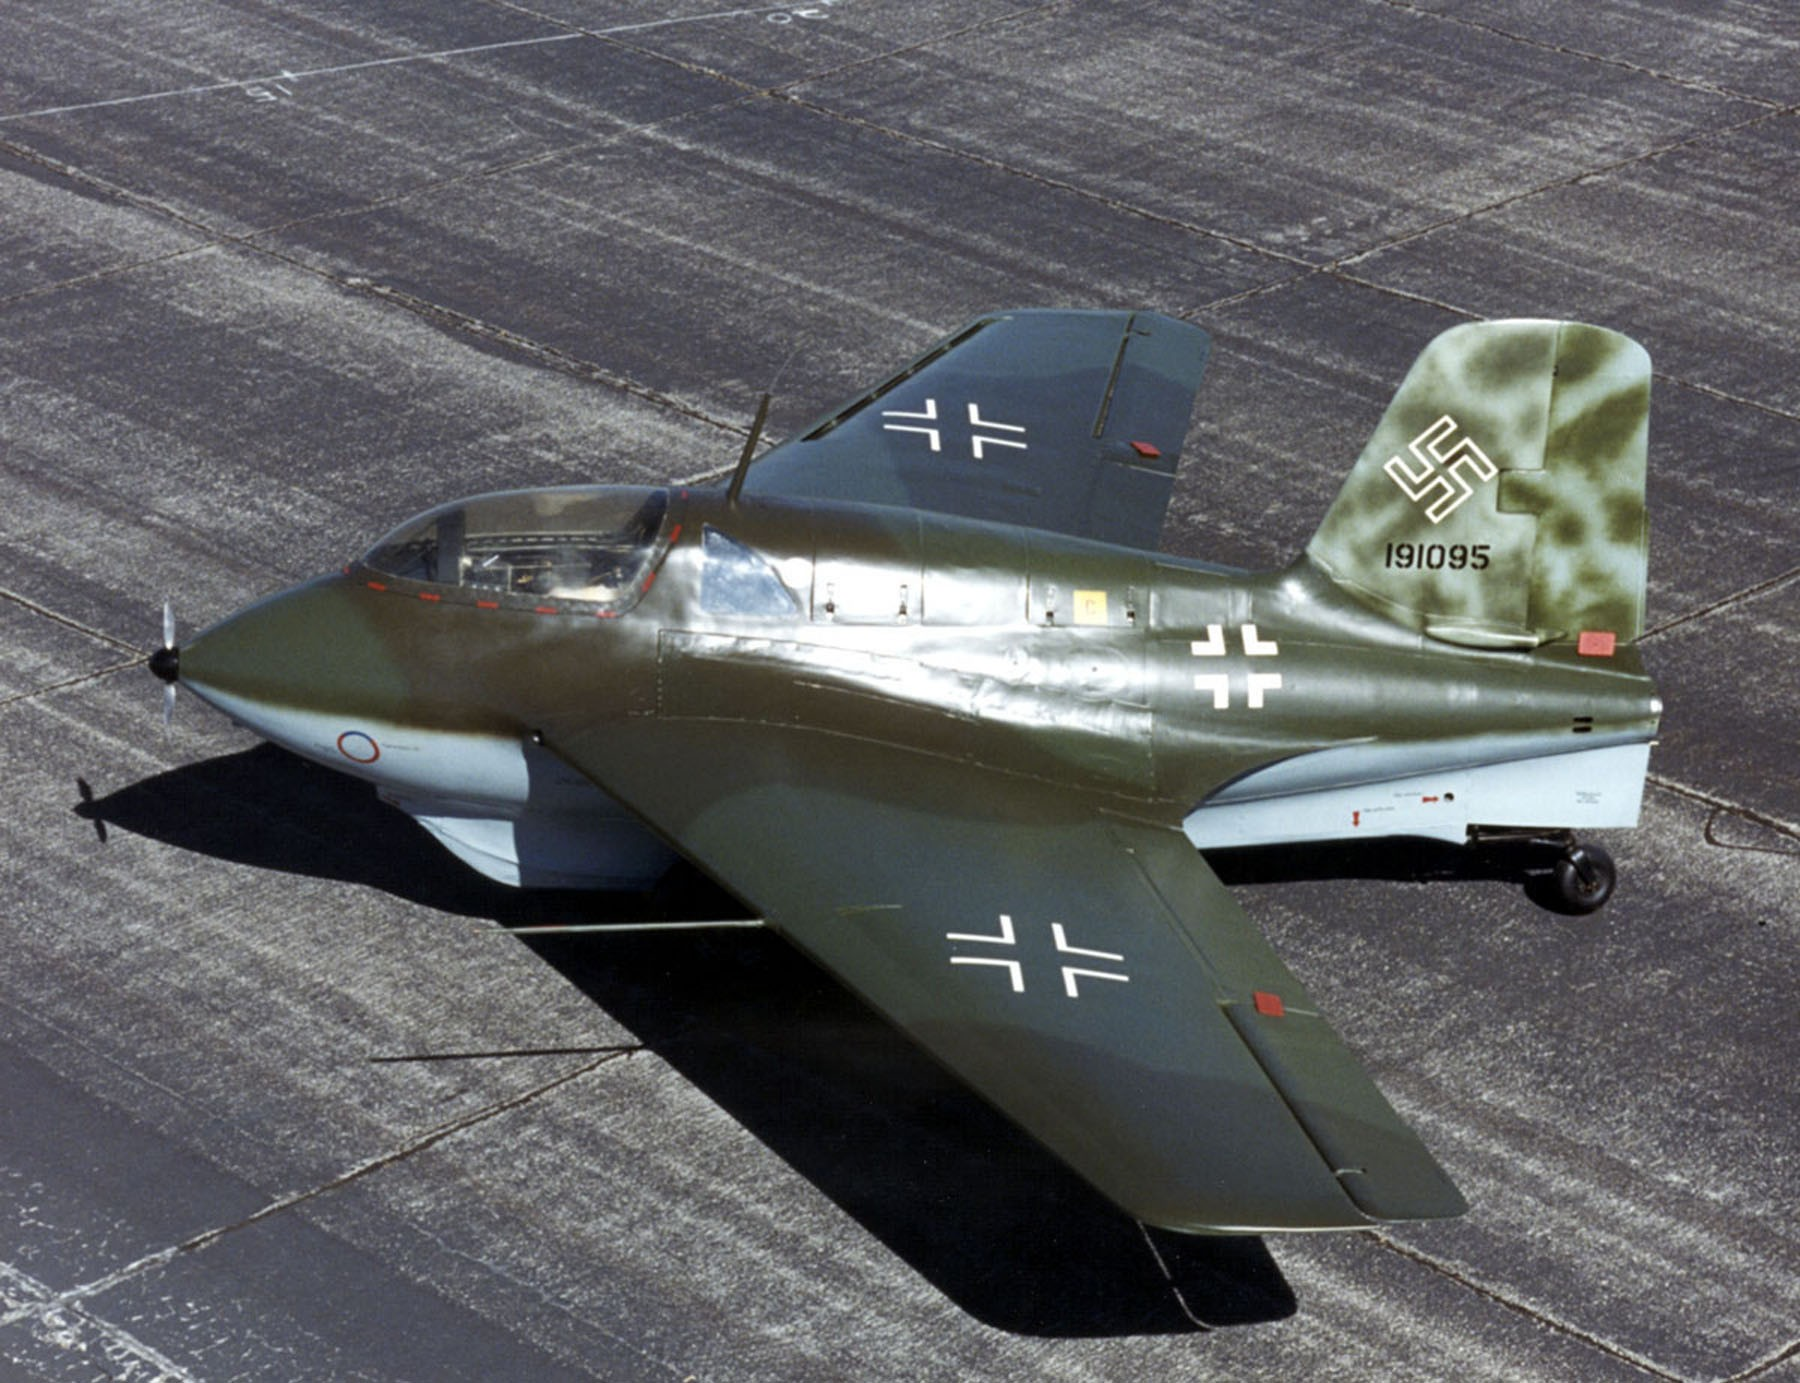
\includegraphics[width = 0.45\textwidth,clip=]{Me163b2}}
  \end{subfigmatrix}
  \caption{\label{FIG_EXAMPLE}Examples of different aircraft propulsion systems: (a) propeller-driven IC-engine: Cessna 350 Corvalis, (b) turbofan engine: Honda HA-420 HondaJet, and (c) rocket-engine: Messerschmitt ME-163 Komet.}
  \end{center}
\end{figure}
%==============================================================================
\vspace*{1in}


